% Chapter 5

\chapter{Workplace for automated data collection.}\label{Chapter5}
\lhead{Chapter 5. \emph{Workplace for automated data collection}}

The workstation described here can automatically measure high
frequency and low-frequency capacitance of the MOS
structure. Figure~\ref{fig:5.1} shows shows the block diagram of the
instruments by which the individual methods are implemented.

\begin{figure}[h!]\centering
  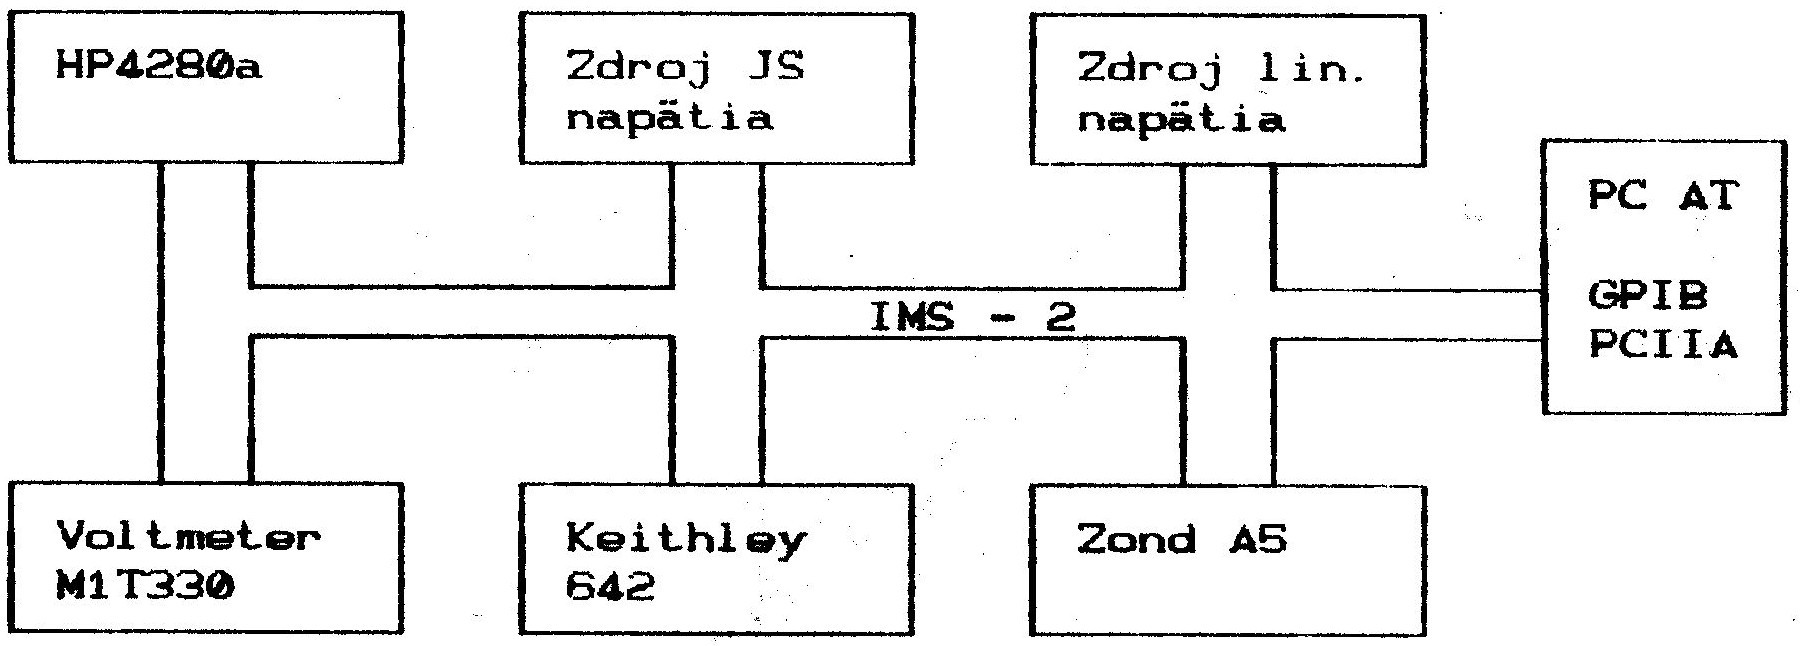
\includegraphics{Figures/fig-5-1.eps}% chktex-file 8
  \caption[Block diagram of automated instrumentation
    workstation]{Block diagram of automated workstation
    instrumentation workstation for determining the area distribution
    of parameters of structures MOS with inhomogeneous substrate
    endowment.}\label{fig:5.1}
\end{figure}

The measurement control computer is a PC AT personal computer equipped
with IMS-2 interface (IEEE 488 standard) from National Instruments
model GPIB-PCIIA, which operates as an IMS-2 bus controller. All
connected instruments are equipped with an IMS-2 interface, which can
be used to to remotely control and collect measured data. In addition
to the professional HP4280a and Keithley 642 measuring instruments
were used in the experiment DC voltage sources and a linearly
increasing voltage source built in the Department of
Microelectronics. The M1T330 voltmeter is a product of Metra Blansko
and the Zond A5 stepping spike device was imported from Soviet
Union. The latter device does not include as standard IMS-2 interface
and was retrofitted with an IMS-2 module of its own design~\cite{5.1}.

Another new feature of our implementation of the structure measurement
workstation MOS is the ability to automatically collect data across
the silicon wafer and their save to a disk file for subsequent
processing. Programming equipment of the workstation can be divided
into (1) data acquisition programs (2) data processing (3) results
display and (4) auxiliary programs. The data acquisition programs
allow the measurement of the C-V dependence in any number of points on
the silicon wafer, the positions of which are selectable and are
defined by the operator.

An important point in the implementation of the data acquisition
programs was to ensure against the loss of measured data due to the
occurrence of arbitrary error (e.g., voltage failure) or in case of
the necessity to interrupt measurement. Because the duration of data
acquisition on a silicon board with 300 structures varies from 0.5 to
12 hours depending on the type of measurement required, it was
necessary to programmatically provide (1) the possibility of
interrupting the measurement by the operator at any point (2) the
possibility of restarting the data collection at the point where the
data was collected interrupted. Ensuring that measured data is
retained in the event of an occurrence of error was implemented as
follows. Measured data are at once written to a disk file each time a
measurement is completed on each structure. This data unit will be
referred to as a record in the following. This means that damage to a
data structure can only occur if the occurrence of an error within a
short period of time (on the order of tens of ms), but this only
results in the loss of the last record. For this case an auxiliary
program is available which truncates the data file to the required
amount of records, thus restoring the compactness of the file and
allowing restart the data collection. In this way, the data file can
be truncated by erroneously measured data even after the operator has
interrupted the data acquisition, if the a fault is detected during
the measurement. At the same time it is available an auxiliary program
that allows overwriting any number of records data file. The
usefulness of this program will be explained in the following example.

Suppose that in the course of the data collection there were
(e.g.\ due to the effects of environmental conditions) an error
occurred that lasted for a short period of time, causing part of the
records of the data set contain erroneous data. An example may be
imperfection of the tip contact with the sample to be measured caused
by vibrations. This is often only detected when the measurement is
evaluated or displayed results. After the positions of the structures
on the silicon wafer under test have been determined, where we have
measured erroneous data, we can measure at these points repeat the
measurement and overwrite the records in the original data file.

Data acquisition programs for HF C-V have been implemented in the
above manner, the quasi-static C-V method, the oxide layer capacitance
measurement and the constant width space charge region. However, we
could not automate the Q-C method because the instrument interface
used by the Keithley 642 does not allow remote control of input
terminal shorting of the measuring instrument, thus making it
impossible to automate the zeroing of the charge in the the common
point of the capacitor connections that gets there due to leakage
currents.

For convenient manipulation of the data files, the following has been
chosen naming concept of the data files. Naming the file in the
operational MS DOS system consists of a file name and a file
extension.  File name represents in our case the name of the measured
silicon wafer and the suffix denotes the type of data the file
contains. In principle, it can be divided into the above data files
into two types according to the data they contain each records. It can
be a functional dependency or a parameter. If it is functional
dependency, then the first record in the data file contains the number
of points at which the functional dependency was captured and the
values of the independent variable values. The next records contain
the position of the structure on the silicon plate, expressed as two
integers (X,Y), the number of points and the functional values.
Repetitive information on the number of points of the functional
dependence is not redundant because in the event of a measurement
failure (e.g.\ a breakthrough) on the (X,Y) structure, it contains the
number -1, which communicates absence of function values in the
record. An example would be HF C-V dependency. The first record
contains the number of capacitance measurements on one structure and
the gate voltage values. The next records contain the position of the
structure (X,Y), the number of points and the capacitance values
corresponding to gate voltages from the first record. Files of the
second type consist of only records containing the structure positions
(X,Y) and the value of parameter value. As an example, consider a data
file that contains capacitances of the oxide layer of the MOS\@
structures. Since this is a large data files, the binary form of the
record has been chosen.  The integer values have 2 bytes in length and
floating point numbers take up 4 bytes.

In case a data file containing data in the form of ASCII, a helper
program is available which, after entering the position of the
structure (X,Y) will create this data file and write the data to it,
containing the record with position (X,Y). If this is a functional
dependency, it also writes the values to the output file in ASCII form
of the independent variable.

\section{Measurement of HF C-V dependencies.}\label{sec:5.1}

We measure the HF C-V dependence of the MOS structure using the
HP4280a instrument, which determines both the capacitance and
conductivity of the sample being measured based on phase shift between
the HF voltage signal (1MHz,30mV) and the measured current. The
HP4280a instrument is equipped with a proprietary processor that
controls its internal functions and provides the operator with
comfortable control. For HF C-V dependence measurement, we need to set
the desired voltage interval, in which to measure the capacitance
(Vstart, Vstop) and the voltage step Vstep, at which the DC voltage
will be varied. The measurement time ratios are are determined by two
other parameters. Thold determines the time during which the the
voltage Vstart is applied to the sample to be measured before the
measurement. This time is required for the transients to settle, in in
case we do not want to measure them. The Tdelay parameter specifies
the dwell time of the measurement after the voltage step has been
performed.

For the automated measurement of the structures, we have chosen the
most powerful mode of the HP4280a, in which, according to the pre-set
parameters automatically performs the entire measurement and stores
the measured data in the internal memory.  The data transfer from the
HP4280a to the control computer is is done in binary form, thus not
wasting time converting between binary and ASCII form, while the
binary form represents a smaller fewer bytes to transfer. Completion
of measurement and readiness for data transfer is indicated by the
HP4280a by setting the SRQ signal (Service Request) signal on the
IMS-2 bus to synchronize its operation with the control computer.  A
useful feature can be mentioned here of the GPIB-PCIIA~\cite{5.2}
interface, which, after detecting the SRQ signal, can automatically
execute a Serial Poll and after locate the instrument that requests
service to store its status word in the internal memory. This frees
the SRQ driver of the IMS-2 bus and the interface GPIB-PCIIA can
respond to service requests from other instruments. If the control
program requests the instrument status word, that has requested
service, the GPIB-PCIIA interface will issue it from its internal
memory.

By using automatic measurement control and binary data transfer, the
the minimum HF C-V measurement time has been achieved.  The specific
values measurement durations and timing diagrams are given in
Section~\ref{sec:5.4}.

If we need to determine the concentration profile of the interfering
impurities in a larger depth than the width of the OPN in the
inversion state, we need to measure the C-V dependence in the deep
depletion state. In this case, always after the stress jump to the
deep depletion state (and measure the capacitance) we must return to
the accumulation state for a certain time. The HP4280a does not have a
mode mode of operation that would automatically control this kind of
measurement. Therefore, we must have to manage each capacitance
measurement independently. Measurement control cycle program then
contains the setting of the desired gate voltage, execution of the
capacitance measurement (starting the measurement and waiting for the
completion) and the transfer of data from the measuring instrument to
the control computer, all of the above transfers are made in ASCII@
form. Compared to to the standard HF C-V method, the length of a
single point C-V measurement depends is increased by orders of
magnitude.

The accuracy of the determination of the concentration profile of the
interfering impurities strongly depends strongly on the accuracy of
the determination of the capacity of the oxide layer.  Therefore the
oxide capacity is determined using a separate program that measures
the capacitance of the MOS structure for a specified gate voltage far
in the accumulation and stores the measured values in a separate data
file.

\section{Measurement of quasi-static C-V dependencies.}\label{sec:5.2}

We measure the quasi-static C-V dependence of the MOS structure using
a source of linearly increasing voltage, a Keithley 642 electrometer
and a voltmeter M1T330. We determine the capacitance of the MOS
structure from the relation

\begin{equation}\label{eq:5.1}
  C_{mos}^{LF} = i\ {\bigg[\frac{dV_{g}}{dt}\bigg]}^{-1}
\end{equation}

Accurate measurement of the charging current of the MOS structure is a
major problem of the quasi-static C-V method. Keithley supplies its
measurement IMS-2 interfaces. In our measurement setup there is model
1793/6423 is used, which, apart from transmitting measured data, does
not perform no other functions and the operation of the instrument has
to be controlled manually from front panel.  Before starting the
measurement it is necessary to set the measured the quantity to be
measured (in addition to current, voltage and charge can also be
measured) and the measuring range of the instrument.

The measurement and data transfer from the electrometer to the control
computer can can be performed in two modes, which differ by the
address instrument~\cite{5.3}. In continuous mode, the A/D converter
operates of the instrument continuously and on request to send data to
the computer the interface sends the last completed measurement (at
this point it may already be the next A/D conversion can be started at
this point). In triggered mode, the A/D converter waits for the
command to start the measurement from the interface, which it receives
after a request from the controller computer to send the measured
data. Then the A/D conversion takes place and the measured data is
sent to the computer. Keithley measurement time 642 is 400 ms. This
time is required for dynamic phenomena to settle, caused by
communication over the IMS-2 bus. Because the interface of the
instrument is not galvanically isolated from the measurement part, the
circuitry has the current measurement circuit and the IMS-2 bus share
a common ground. Thus, the bus communication IMS-2 bus communication
during A/D conversion causes the measured signal to be noisy.  This
problem can be eliminated by using a triggered mode in which the
instrument, after receives a request to transmit measured data, it
first waits for the measured data to stabilize dynamic phenomena and
then performs the A/D conversion.

In addition to the current, we need to know the slew rate to calculate
the capacitance voltage at the gate of the MOS structure, which we
determine as follows.  We will perform the measurement in a larger
voltage range than required. V start and end section (outside the
required voltage interval) measure the values of the linearly
increasing gate voltage and at the same time measure the time for each
voltage value. We measure the time by internal control computer clock
with a resolution of 1/12 s. By linear regression of the sampled data
to determine the $V_{g}(t)$ dependence directive, which we use in the
capacity calculation.

As mentioned earlier the current measurement takes 400 ms.  In order
to get the as many measured C-V dependence points as possible, we have
chosen the following procedure to determine the gate voltage
corresponding to the measured current. Simultaneously with the
measurement of the current, we subtract the elapsed time from the
start of the measurement and the gate voltage is calculated using the
$V_{g}(t)$ dependence directive. Subtraction and storage of the
elapsed time is a fast operation of the control computer, thus we gain
the time that would have been lost by measuring the voltage using
voltmeter. Another advantage of the above procedure is that we get a
smoothed values of the gate voltage waveform over time. In the case
where we would have measured both current and voltage directly, we
would get error-laden measurements of both both the functional values
and the values of the independent variable, which could cause problems
in smoothing the measured data.

Although the measurement of current and time is automatic in the
measuring loop, we may not always obtain a C-V dependence with an
equidistant step in the voltage axis and we also cannot determine in
advance at what gate voltage we measure the capacitance.
Preprocessing of measured data before writing to a disk file therefore
consists of an approximation of the C-V dependence using cubic spline
functions and calculating the capacitance of the MOS structure for the
specified voltage values. It is necessary to select the values gate
voltages in accordance with the HF C-V measurement, which will
facilitate the calculation of those parameters of MOS structures that
are determined from HF and quasi-static C-V dependence.

\section{Constant width method OPN measurement.}\label{sec:5.3}

For the constant-width OPN measurement, we used the instruments
HP4280a and a direct current (DC) voltage source, which was built on
Department of Microelectronics. The measurement circuit of the HP4280a
instrument consists of an internal JS voltage source (INT BIAS), an HF
signal source and ammeter (denoted by A)~\cite{5.7}. The internal JS
voltage source has a range of $(-100.0,+100.0)V$ with a resolution of
$0.1V$, but a range of $(-2.0,+2.0)V$ we can set the voltage with a
resolution of $0.001V$. If we are measuring MOS structures formed on
high quality silicon substrates, the relaxation of non-equilibrium
charge carriers is slow, causing also causes a slow change in the
capacitance of the MOS structure.  In order to be able to maintain
constant size of the non-equilibrium capacitance of the MOS structure,
we need change the gate voltage as little as possible. For this
purpose, a voltage range of (-2.0,+2.0) V of the internal JS source of
the HP4280a instrument. To bring the MOS structure into
non-equilibrium state of deep depletion, we use an external JS voltage
source that can adjust the voltage in the range (-40.0, +40.0) V with
a resolution of 0.1 V. The HP4280a instrument allows great flexibility
in element configuration of the measuring circuit. 14 modes are
available. For our experiment, we we chose mod 11~\cite{5.2}, which
allows the connection of an external power supply JS voltage source.

\begin{figure}[h!]\centering
  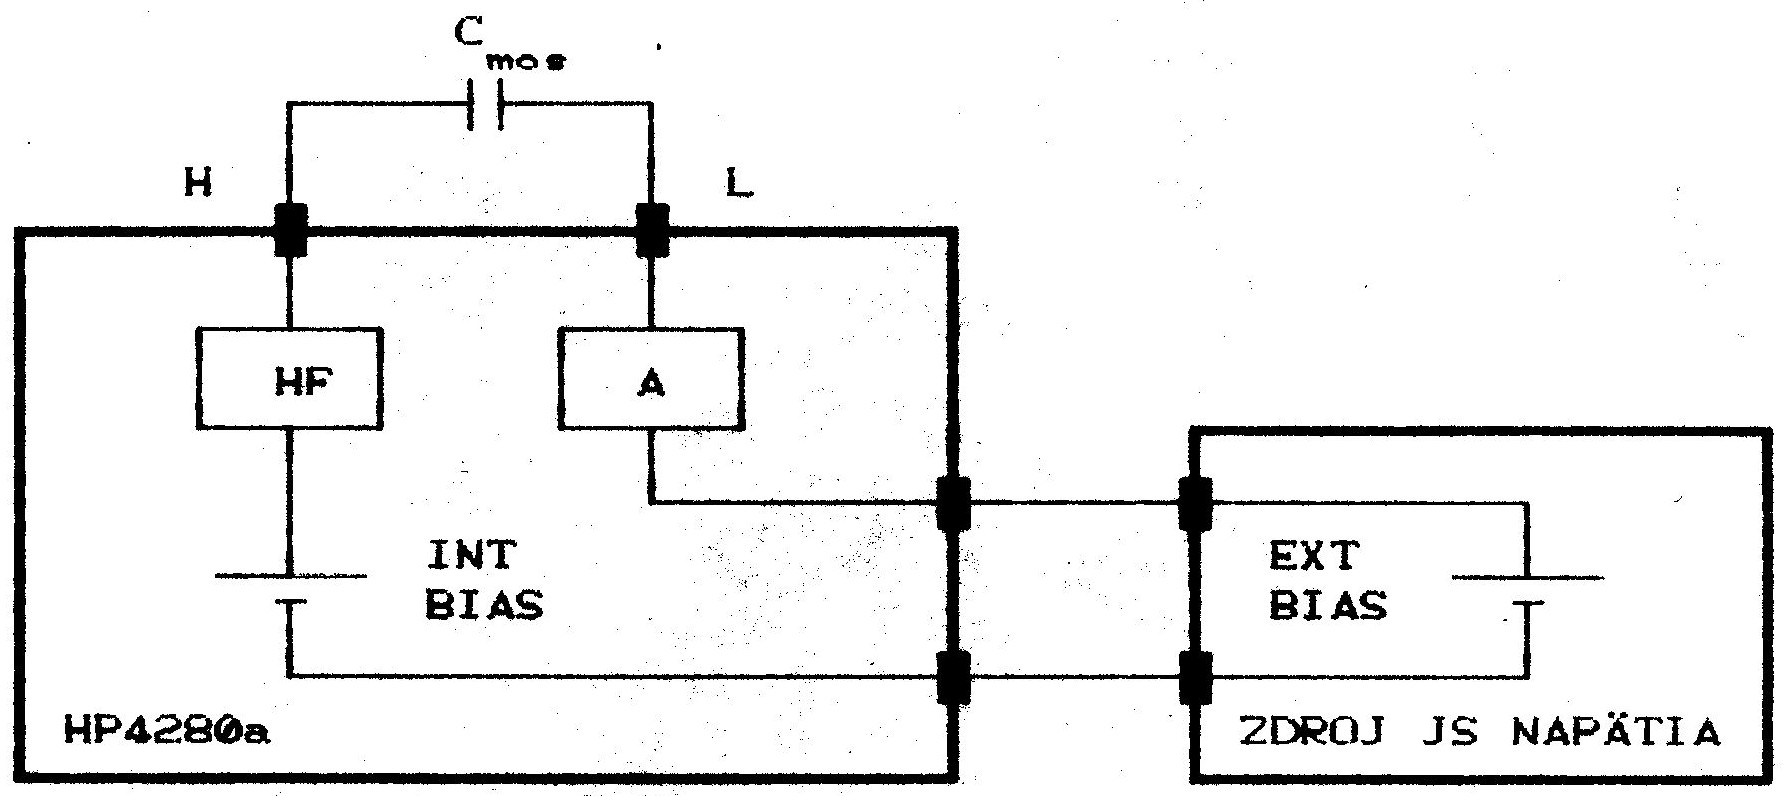
\includegraphics{Figures/fig-5-2.eps}
  \caption[Instrument wiring for constant width method
    OPN]{Instrument connection for constant width method
    OPN.}\label{fig:5.2}
\end{figure}

The measurement of the $V_{g}(t)$ dependence then proceeds as follows
steps. Using an external JS voltage source, we bring the MOS structure
to a non-equilibrium state. From the capacitance change ${Delta{C}}$,
which we measure with the HP4280a instrument, we calculate using the
relation~\ref{eq:3.9} the required gate voltage change
$\Delta{V_{g}}$. If its magnitude is v absolute value is greater than
$0.001 V$, we change the value of the gate voltage by $\Delta{V_{g}}$,
thus keeping the value of the non-equilibrium capacitance of the MOS
structure. For each gate voltage change, we subtract the time when
this change occurred. We stop measuring the dependence $V_{g}(t)$,
when the measurement time (let us denote it by $T_{hold}$) specified
by the operator has elapsed, or if the change in gate voltage has
exceeded the threshold values of the interval $(-2.0,+2.0) V$.
Experimentally, it has been shown that the program feedback loop
ensuring a constant value of capacitance works fast and accurate
enough. During the experiments carried out, the the variation of the
maintained capacitance was better than 1\%.

We repeat the measurement for different values of the capacitance of
the MOS structure in non-equilibrium state to determine the generation
time of the minority charge carriers according to the
relation~\ref{eq:3.10}.

The parameters of the control program are the interval over which to
OPN boundary $(W_{start}, W_{stop})$ with step $W_{step}$. Another
parameter is the value of $T_{hold}$, which gives the maximum
measurement time of one dependency $V_{g}(t)$.

The control program requires data files with measured C-V dependences
of the deep depletion and oxide layer capacities of the tested silicon
wafer structures. Using these pre measured data and from the specified
OPN boundary distance, it then determines the initial gate voltage for
setting the external JS source voltage.  For its operation, the
control program needs one more data file containing the concentration
profiles of the contributing impurities of the measured MOSň2
structures. The concentration values are needed for quantifying the
change in gate voltage of the MOS structure according to
relation~\ref{eq:3.9}.

After measuring the dependence $V_{g}(t)$, we determine by linear
regression its directive. From the experiments carried out, it turns
out that the minimum time dependence measurement $V_{g}(t)$ where one
can still expect an acceptable results is on the order of
$10^{3}\mu{s}$ for substrates with values of $\tau_g$ approximately
$T_{hold}=10s$. During this time, the change in voltage of the gate in
the range of $50-500 mV$ depending on the width of the OPN and
depending the minority carrier contribution from outside the OPN@. At
the same time, the graphical representation of the dependence
$\frac{dV_g}{dt}=f(w)$ shows the influence of of the minority charge
carrier increment from outside the OPN region, which manifested by an
approximately equal slope of the dependence $\frac{dV_g}{dt}=f(w)$,
but with a different absolute value. From the display of the
dependence $\frac{dV_g}{dt}=f(w)$ over the whole silicon slab shows
that acceptable values of $\tau_{g}$ can only be calculated from the
derivative function $\frac{dV_g}{dt}=f(w)$ by w
(relation~\ref{eq:3.10} or~\ref{eq:3.7}) and in any case not from its
functional values (relation~\ref{eq:3.5}). In the output data file we
stored functional dependencies $\frac{dV_g}{dt}=f(w)$.

The principle of the method implies a minimum distance from the
semiconductor surface, in which $\tau_{g}$ can be determined. This
limit is the width of the OPN corresponding to the onset of weak
inversion in the semiconductor.

\section{Time diagrams of the methods used.}\label{sec:5.4}

In order to estimate the measurement time for each method, we show
graphically the time dependence of the gate voltage of the MOS
structure. In addition to the equilibrium HF C-V method, where the
whole measurement waveform is controlled by by the HP4280a instrument
processor and its time diagram is taken from the Manual~\cite{5.7},
the time diagrams were determined based on experimentally measured
values. These time values are dependent on the type of control
computer and on the optimization of the control programs. V our
experiment, we used a PC AT personal computer, operating on 10 MHz
with an 80287 coprocessor (6 MHz) and a hard disk with a access time
of 28 ms. The control programs were compiled without optimization for
speed using an emulation library of subroutines for mathematical
floating point operations.

In conjunction with the timing diagrams, we also provide the voltage
ranges used of the instruments.

\par\emph{NOTE.} In the case where, at the maximum value of the time
`unlimited' is given at the maximum time value, it means that its
maximum size depends on the data type of the corresponding control
variable of the program, or on the range of the instrument.

\newpage
\subsection{Equilibrium HF C-V dependence.}\label{sec:5.4.1}

\begin{figure}[h!]\centering
  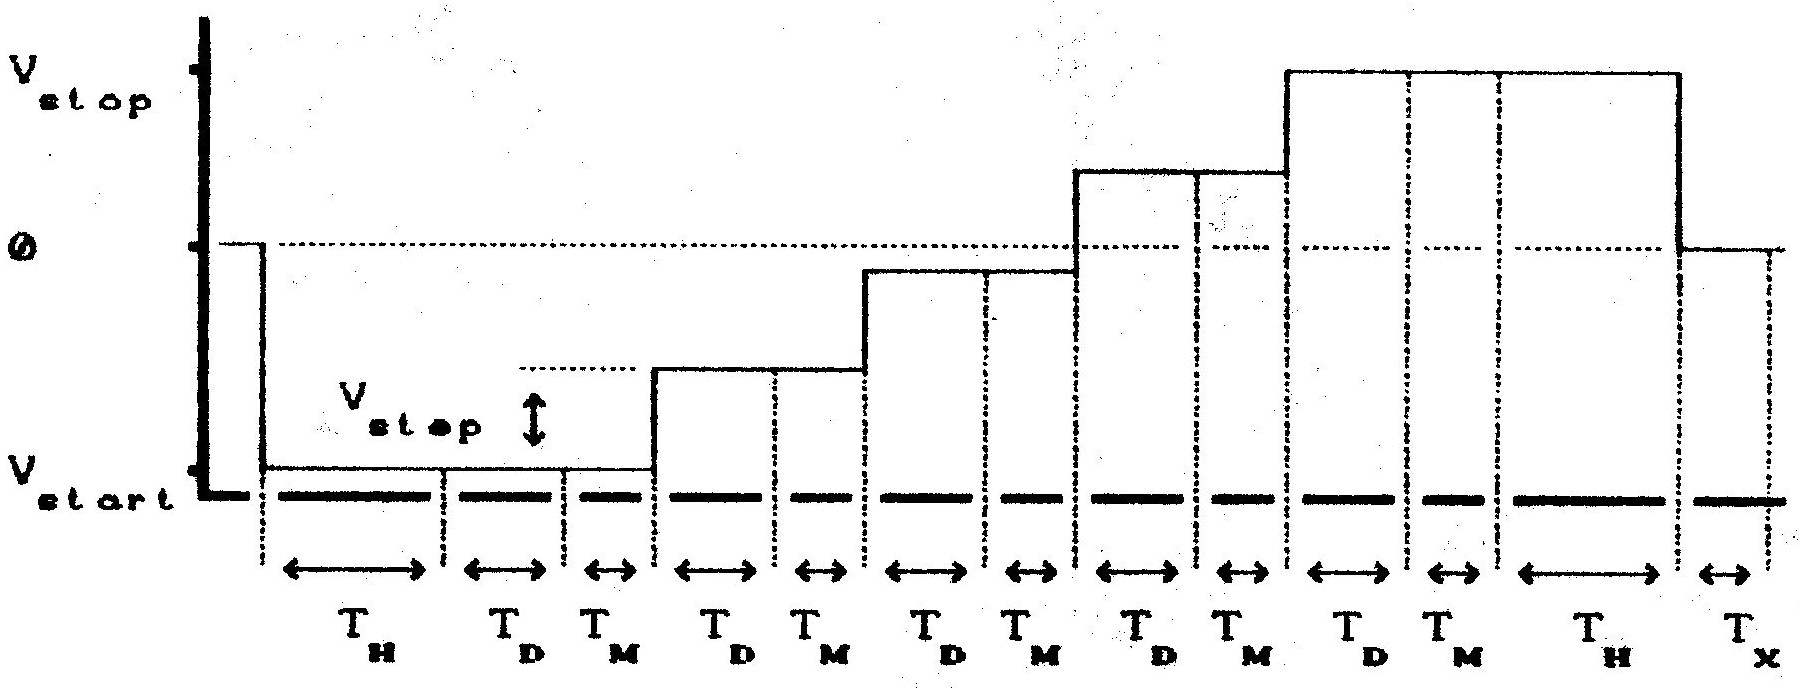
\includegraphics{Figures/fig-5-3.eps}
  \caption[Time diagram of equilibrium HF C-V method]{Time diagram of
    the equilibrium HF C-V method.}\label{fig:5.3}
\end{figure}

\begin{table}[h!]\centering
  \begin{tabular}{l p{0.5\linewidth} l l}
    param.      & parameter description & min. & max.value\\
    \hline% chktex-file 44
    $T_H$       & settling time \dotfill & $3 ms$ & $650 s$\\
    $T_D$       & measurement hold time \dotfill & $3 ms$ & $650 s$\\
    $T_M$       & measurement time \dotfill & $40 ms$\\
    $T_X$       & binary data transfer,\\
                & data preprocessing,\\
                & saving data to file,\\
                & shift table to next structure \dotfill & $\sim 7 s$\\
    $V_{start}$ & \dotfill & $-100.0 V$ & $+100.0 V$\\
    $V_{stop}$  & \dotfill & $-100.0 V$ & $+100.0 V$\\
    $V_{step}$  & \dotfill & $\pm 0.001 V$ & $\pm 200.0 V$\\
    \hline
  \end{tabular}
  \caption[Time diagram of equilibrium HF C-V method]{Time diagram of
    the equilibrium HF C-V method.}\label{tab:5.1}
\end{table}

\newpage
\subsection{Equilibrium HF C-V dependence.}\label{sec:5.4.2}

\begin{figure}[h!]\centering
  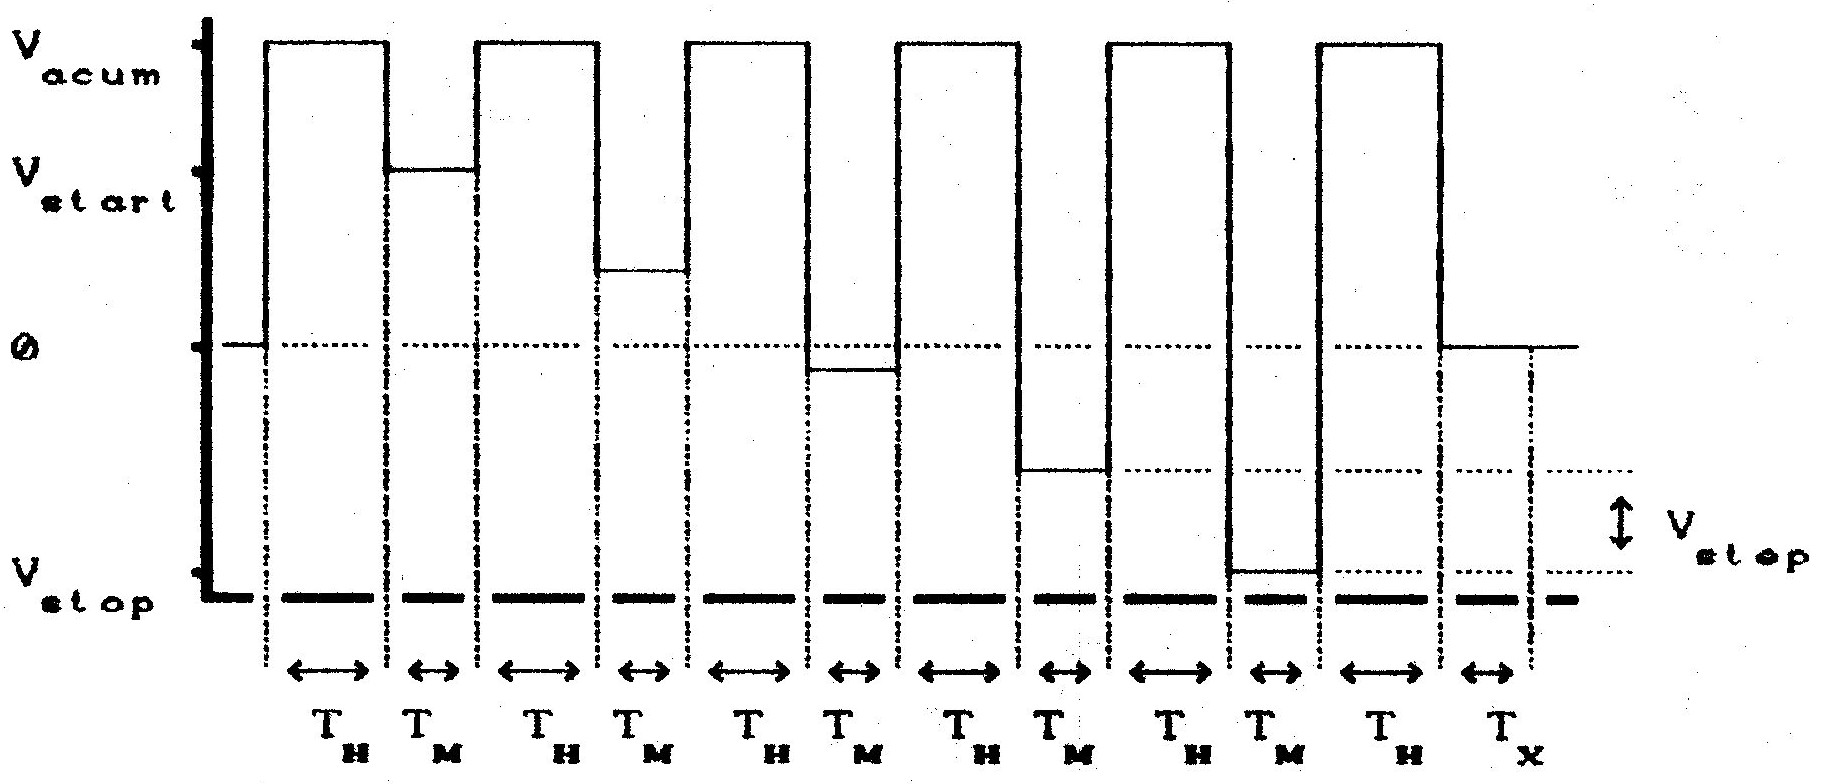
\includegraphics{Figures/fig-5-4.eps}
  \caption[Time diagram of non-equilibrium HF C-V method]{Time diagram
    of the non-equilibrium HF C-V method.}\label{fig:5.4}
\end{figure}

\begin{table}[h!]\centering
  \begin{tabular}{l p{0.5\linewidth} l l}
    param.      & parameter description & min. & max.value\\
    \hline
    $T_H$       & relaxation time of minority charge carriers \dotfill & $0 s$ & unbounded\\
    $T_M$       & data measurement and transfer \dotfill & $330 ms$\\
    $T_X$       & data preprocessing,\\
                & saving data to file,\\
                & shift table to next structure \dotfill & $\sim 4s$\\
    $V_{start}$ & \dotfill & $-100.0$ & $+100.0 V$\\
    $V_{stop}$  & \dotfill & $-100.0$ & $+100.0 V$\\
    $V_{step}$  & \dotfill & $\pm 0.001$ & $\pm 200.0 V$\\
    $V_{acum}$  & \dotfill & $-100.0$ & $+100.0 V$\\
    \hline
  \end{tabular}
  \caption[Time diagram of non-equilibrium HF C-V method]{Time diagram
    of the non-equilibrium HF C-V method.}\label{tab:5.2}
\end{table}

\newpage
\subsection{Quasi-static C-V dependence.}\label{sec:5.4.3}

\begin{figure}[h!]\centering
  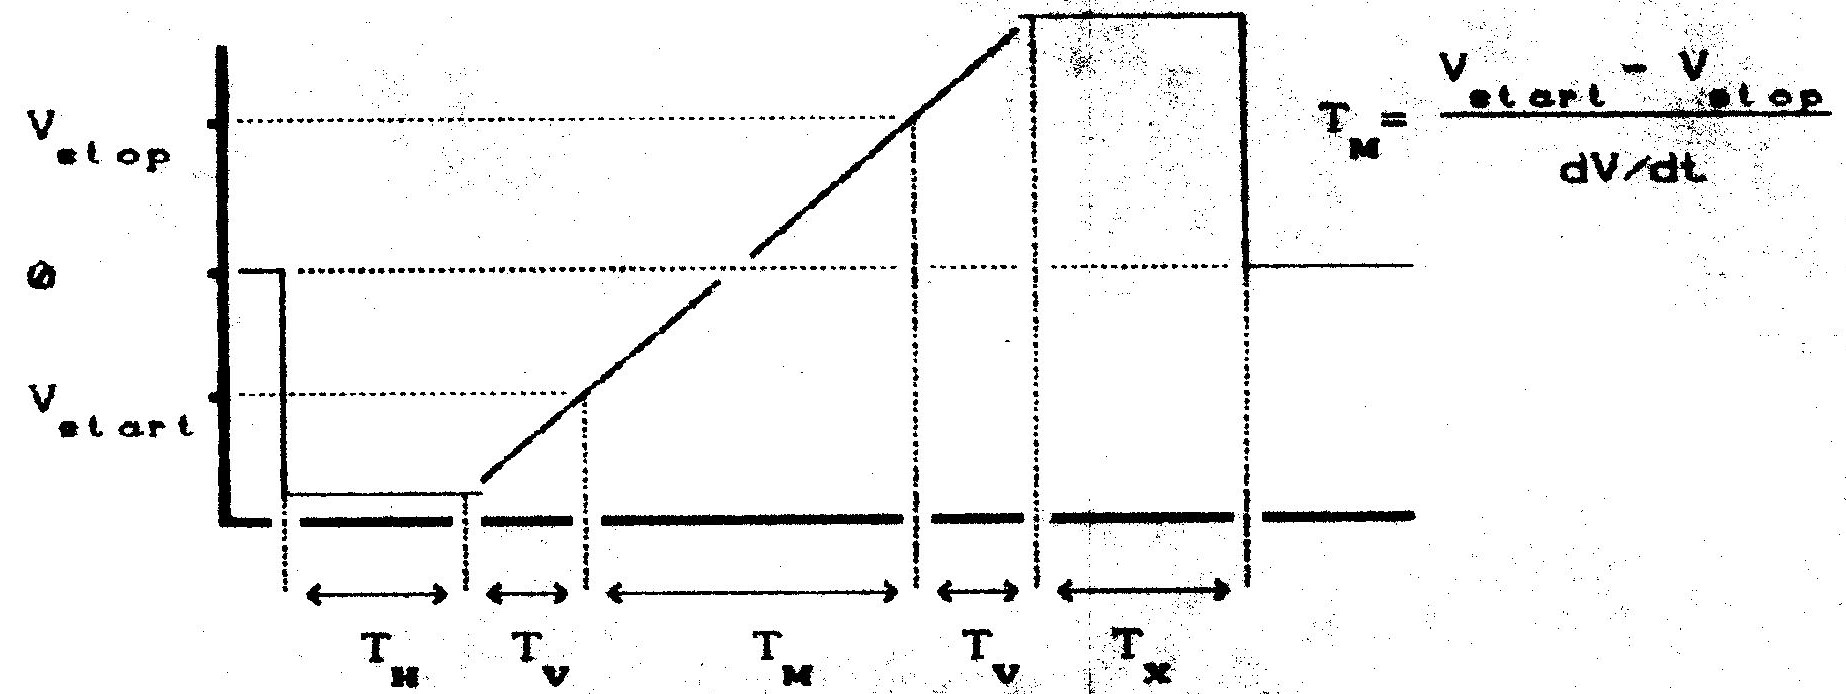
\includegraphics{Figures/fig-5-5.eps}
  \caption[Time diagram of the quasi-static C-V method]{Time diagram
    of the quasi-static C-V method.}\label{fig:5.5}
\end{figure}

\begin{table}[h!]\centering
  \begin{tabular}{ l p{0.5\linewidth} l l }
    param.      & parameter description & min. & max.value\\
    \hline
    $T_H$       & settling time \dotfill & $0 s$ & unbounded\\
    $T_V$       & measurement of gate voltage and time \dotfill & $5s$\\
    $T_M$       & measurement of current and time \dotfill & unbounded\\
    $T_X$       & data preprocessing,\\
                & saving data to file,\\
                & shift table to next structure \dotfill & $\sim 15s$\\
    $V_{start}$ & \dotfill & $-20.0$ & $+20.0 V$\\
    $V_{stop}$  & \dotfill & $-20.0$ & $+20.0 V$\\
    $dV/dt$     & \dotfill & $\pm 0.1mV/s$ & $\pm 10.0V/s$\\
    \hline
  \end{tabular}
  \caption[Time diagram of the quasi-static C-V method]{Time diagram
    of the quasi-static C-V method.}\label{tab:5.3}
\end{table}

\newpage
\subsection{Constant width OPN method.}\label{sec:5.4.4}

\begin{figure}[h!]\centering
  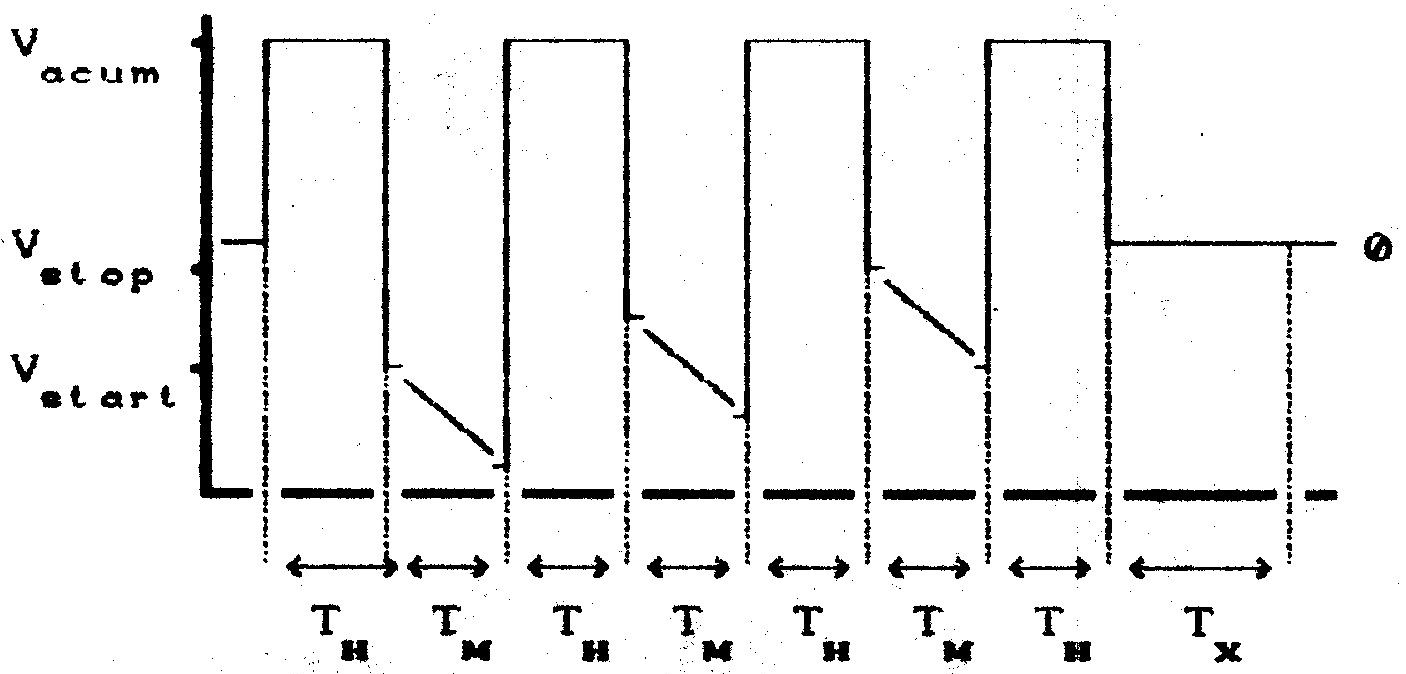
\includegraphics{Figures/fig-5-6.eps}
  \caption[Time diagram of constant width OPN method]{Time diagram of
    the constant width OPN method}.\label{fig:5.6}
\end{figure}

\begin{table}[h!]\centering
  \begin{tabular}{ l p{0.5\linewidth} l l }
    param.      & parameter description & min. & max.value\\
    \hline
    $T_H$       & relaxation time of minority charge carriers \dotfill & $0 s$ & unbounded\\
    $T_M$       & measurement time, calculation of $dV/dt$ \dotfill & $10 s$ & unbounded\\
    $T_X$       & save data to file,\\
                & shift table to next structure \dotfill & $\sim 2s$\\
    $V_{start}$ & \dotfill & $-40.0$ & $+40.0 V$\\
    $V_{stop}$  & \dotfill & $-40.0$ & $+40.0 V$\\
    $V_{acum}$  & \dotfill & $-40.0$ & $+40.0 V$\\
    \hline
  \end{tabular}
  \caption[Time diagram of constant width OPN method]{Time diagram of
    the constant width OPN method.}\label{tab:5.4}
\end{table}


\begin{thebibliography}{}
\bibitem[5.1]{5.1} Mariassy P.: Control unit of the instrument type
  talker/listener for connection to the IMS bus. Thesis. EF SVST
  Bratislava 1988.
\bibitem[5.2]{5.2} National Instruments, IEEE-488 Instrumentation
  Interface. User guide.
\bibitem[5.3]{5.3} Keithley model 642, Instruction manual.
\bibitem[5.4]{5.4} Marchuk G.I.: Methods of numerical
  mathematics. Academia Prague 1987.
\bibitem[5.5]{5.5} Cox M.G.: J. Inst. Maths. Aplics., 10 (1972) p.134.
\bibitem[5.6]{5.6} De Boor C.: J. Approx. Theory, 6 (1972) p.50.
\bibitem[5.7]{5.7} Hewlett-Packard, Operational and service manual,
  Model HP4280a.
\end{thebibliography}
